\chapter{Introdução}

Este capítulo está dividido em quatro seções. A seção 1.1 apresenta a motivação para realização deste trabalho. A seção 1.2 descreve o problema a ser tratado nesta dissertação. A seção 1.3 mostra as questões que nortearam esta pesquisa. A seção 1.4 os objetivos e o escopo deste trabalho. Por fim, a seção 1.5 descreve a estrutura segundo a qual este trabalho está organizado.

%Este é um relatório técnico \cite{BON03}, um livro \cite{SILBERSCHATZ}, um relatório técnico \cite{PIERCE}, referência da Web \cite{DB2XML}, trabalho de final de curso \cite{Angelo}, e tese de doutorado \cite{HAR98}.

%Artigo sem ano \citet{SPH03}.
%Artigo sem ano \citet{SPH03}.  \\
Artigo sem ano \citet{Longuet-1950}.   \\
%\citet{Hou95} \\
%\citeauthor{Hou95} \\
%\citeonline{Hou95}
Em \citep{SPH_LIU_2003}
Em \cite{Scan-1990-Blelloch}

\section{Motivação}

%Uma seção...

%Agora vamos referenciar a Figura \ref{figuraEPS}.

A criação manual de Casos de Teste por vezes é muito trabalhosa, sendo uma tarefa que compromete tempo e recursos por parte dos Analistas de Teste (SOUSA, 2009). Além disso, o trabalho de criação manual dos casos de teste pode ser considerado uma tarefa entediante (ISMAIL, 2007), o que pode afetar a forma como os testes são planejados e construídos. Dessa forma o analista de teste pode não alcançar uma cobertura de restrições positivas e negativas satisfatórias prejudicando a qualidade esperada para o software (SILVA-DE-SOUZA, 2012).

Com o passar dos anos a preocupação com relação à qualidade do software aumenta consideravelmente a medida que a complexidade dos sistemas evolui (SILVA-DE-SOUZA, 2012). Ao escolher uma abordagem orientada a Modelos uma parte desta complexidade é abstraída do desenvolvimento e o analista passa a ter a chance de criar os seus modelos de teste independentemente da plataforma utilizada, gerando maior portabilidade entre os sistemas da informação (BRAMBILLA, CABOT E WIMMER, 2012). A possibilidade de automatizar a criação de variados procedimentos de testes a partir de um simples modelo em alto nível de abstração torna o desenvolvimento mais veloz, menos dependente de tecnologia e sem necessidade de conhecimento profundo em determinada linguagem de programação, diminuindo a quantidade de recursos superutilizados, tempo, custo e aos riscos aos quais o desenvolvimento está sujeito (SOUSA, 2009). Ao possibilitar que a criação dos casos de teste seja realizada de forma automática diretamente a partir de diagramas de classe que expressem o domínio e suas regras de negócio, pode-se então diminuir o tempo e os recursos gastos durante o desenvolvimento.

\section{Problemática}

Segundo Sousa (2009) os maiores esforços durante o ciclo de desenvolvimento de um software se concentram na fase de teste, que chegam a atingir cerca de 50 /percent ou mais dos custos de desenvolvimento de software (XU et al, 2015). Nesta fase é notado um grande desperdício de tempo, custo e recursos por parte das desenvolvedoras. Além disso, a construção manual dos casos de teste acaba por generalizar eventuais erros humanos, abrindo possibilidade para que defeitos se propaguem durante todo o desenvolvimento afetando diretamente a qualidade do produto final (SOUSA, 2009).

\section{Objetivo do Trabalho}

O objetivo geral deste trabalho é definir uma abordagem que possibilite a geração automática de casos de teste para independentes de plataforma a partir de modelos de classes UML enriquecidos com restrições OCL.

\section{Organização do Trabalho}

Esta dissertação está organizada em sete capítulos. O capítulo 1 mostrou a introdução do trabalho, ressaltando a sua motivação, o problema tratado e seus objetivos. O capítulo 2 discorre sobre o referencial teórico deste trabalho, através de um resumo da revisão bibliográfica. O capítulo 3 apresenta a abordagem proposta, através de um exemplo simples. O capítulo 4 descreve a metodologia aplicada para colher indícios da utilidade da abordagem proposta e responder as perguntas da pesquisa. O capítulo 5 apresenta os resultados obtidos após a utilização da metodologia, e por fim o capitulo 6 conclui a dissertação, apresentando as considerações finais, contribuições e sugestões de trabalhos futuros. Em seguida, é apresentada a lista de referências bibliográficas utilizadas. Finalmente, são apresentados na forma de apêndices os instrumentos utilizados no estudo quasi-experimental.

%\begin{figure}
   %\begin{center}
     %\scalebox{0.5}{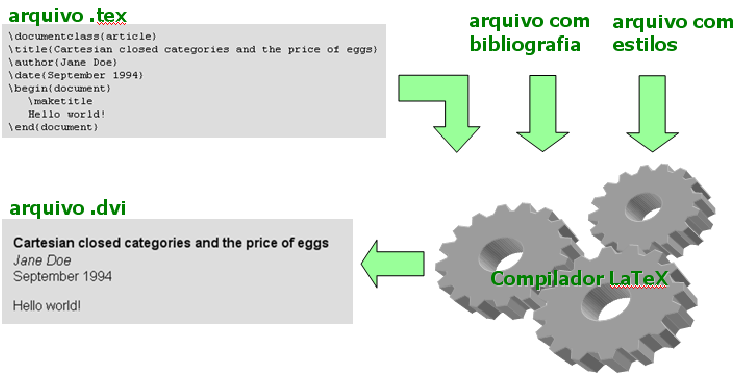
\includegraphics{figs/figuraTeste}}
   %\end{center}
   %\caption{Testando uma figura...\label{figuraEPS}}
%\end{figure}


%\subsection{Bla blá}

%Uma subseção...

%\subsubsection{ABC}

%Uma subsub-seção.
